\documentclass{article}

\usepackage{graphicx} % Required for inserting images
\usepackage{hyperref}
\usepackage{amsmath}
\usepackage{amsfonts}
\usepackage{enumitem}
\usepackage{dsfont}
\graphicspath{ {./images/} }

\title{Introduction to Quantum Information and Computing Half 2 Lecture 5}
\author{Shrikara A, Arnav Negi, Kriti Gupta, Manav Shah, Mohammed Shamil,\\ Shiven Sinha, Swayam Agarwal, Vineeth Bhat, Yash Adivarekar}
\date{17th February, 2023}

\begin{document}

\pagenumbering{gobble}
    \maketitle
    \vfill
    Some Convention: 
    \begin{itemize}
        \item $H$ denotes the Hadamard gate
        \item $U_f$ and $C_f$ have been used interchangeably. 
    \end{itemize}
    \tableofcontents
    \pagenumbering{arabic}
    \newpage

    \section{Phase Kickback Oracle}
    Consider the CNOT gate where $U_f$ denotes the unitary operation CNOT.\\
    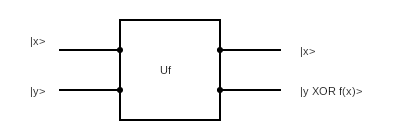
\includegraphics{images/CNOT.png}
    The action of $U_f$ is given by:  
    \begin{align*}
    |x\rangle|y\rangle \xrightarrow{U_f} &|x\rangle|y\rangle \text{ if }f(x)=0\\
    & |x\rangle|\overline{y}\rangle \text{ if }f(x)=1\\
    \end{align*}
    $|x\rangle,|y\rangle \in \{0,1\}$
\\
\\
    Consider the case when $|y\rangle=|-\rangle$
    \begin{align*}
    |x\rangle|-\rangle \xrightarrow{U_f} &U_f\frac{(|x\rangle|0\rangle+|x\rangle|1\rangle)}{\sqrt{2}}\\
    =&\frac{|x\rangle(|0 \oplus f(x)\rangle +|1 \oplus f(x)\rangle)}{\sqrt{2}}\\
    =&|x\rangle|-\rangle \text{ if } f(x)=0\\
    &-|x\rangle|-\rangle \text{ if } f(x)=1\\
    =&(-1)^{f(x)}|x\rangle|-\rangle
    \end{align*}
\\
\\
    If $x \in \{0, 1\}^n$ and before $U_f$, $H^{\otimes n}$ is applied on $|x\rangle$, then the output is:
    \begin{align*}
    &U_f \frac{1}{\sqrt{2^n}}\sum_{z \in \{0,1\}^n} |z\rangle|-\rangle && \textit{from the action of H}\\
    &=\frac{1}{\sqrt{2^n}}\sum_{z \in \{0,1\}^n} (-1)^{f(x)} |z\rangle |-\rangle && \textit{from the action of $U_f$}
    \end{align*}

    Usually, the $|-\rangle$ in the second register is dropped when writing the phase kickback since it remains unchanged in output and is considered implicit when using the phase kickback oracle.

    \section{Deutsch Algorithm}
    \subsection{The Problem}
    Suppose $U_f$ is given as a black box for a boolean function $f: \{0,1\} \rightarrow \{0,1\}$, with the promise that either:
        \begin{enumerate}[label=(\roman*)]
            \item $f(0)=f(1)$
            \item $f(0) \neq f(1)$
        \end{enumerate}
    How many queries do we need to make to $U_f$ to determine which of the two is true?  
    \subsection{Classical Reversible Computation}
    Classically, two queries to $U_f$ are needed, one to determine the value of $f(0)$ and one to determine the value of $f(1)$. We can then compare the two and decide which promise is true.
    %%! put images here
    \\\\images of classical circuit\\

    \subsection{Quantum Computation}
    Consider the following quantum circuit:\\
    %%! put image here
    \\\\image of quantum circuit\\\\\\

    \subsubsection{Finding Final State}
    Finding the output: \\
    \begin{align*}
        |0\rangle|-\rangle \xrightarrow{H \otimes \mathbb{I}} &|+\rangle|-\rangle  && \textit{Apply H to first register} \\
        \xrightarrow{U_f} &\frac{1}{\sqrt{2}} ((-1)^{f(0)}|0\rangle + (-1)^{f(1)}|-\rangle) |-\rangle && \textit{Apply phase kickback}\\
        \xrightarrow{H \otimes \mathbb{I}} &\frac{1}{\sqrt{2}} ((-1)^{f(0)}|+\rangle + (-1)^{f(1)}|-\rangle) |-\rangle && \textit{Apply H to first register}\\
        =&\frac{1}{\sqrt{2}} \left( \frac{(-1^{f(0)})(|0\rangle + |1\rangle)}{\sqrt{2}} + \frac{(-1^{f(1)})(|0\rangle - |1\rangle)}{\sqrt{2}}\right)|-\rangle \\
    \end{align*}

    By rearranging terms containing $|0\rangle$ and $|1\rangle$, we obtain the final state $|\psi\rangle$ as
    \begin{align*}
        |\psi\rangle=\frac{1}{2} \left( ((-1)^{f(0)} + (-1)^{f(1)})|0\rangle + ((-1)^{f(0)} - (-1)^{f(1)})|1\rangle \right)
    \end{align*}
    Note that the $|-\rangle$ in the second register has been dropped since it is implicit for a phase kickback oracle.

    \subsubsection{Probability Distribution}
    The probabilities of the final states being $|0\rangle$ and $|1\rangle$ can be calculated from the square of the corresponding amplitudes of $|0\rangle$ and $1\rangle$, giving
    \begin{align*}
        &\mathds{P}(|0\rangle) = \frac{1}{4} \left( (-1)^{f(0)} + (-1)^{f(1)} \right) ^2 \\
        &\mathds{P}(|1\rangle) = \frac{1}{4} \left( (-1)^{f(0)} - (-1)^{f(1)} \right) ^2 \\
    \end{align*}

    \subsubsection{Resolving a Promise}
    To resolve which one of the two promises are true, we measure the final state.
    If $f(0)=f(1)$
    \begin{align*}
        & \langle 0 | \psi \rangle = 1\\
        & \langle 1| \psi \rangle = 0\\
    \end{align*}

    If $f(0)\neq f(1)$
    \begin{align*}
        & \langle 0 | \psi \rangle = 0\\
        & \langle 1| \psi \rangle = 1\\
    \end{align*}
    Thus, if the final state is orthogonal to $|1\rangle$, then $f(0)=f(1)$ and if it is orthogonal to $|0\rangle$, then $f(0) \neq f(1)$. \\

    \subsubsection{Comparison}
    We observe that the quantum computer needs only $1$ query while the classical reversible computer needed $2$ queries to $U_f$. 

    \section{Deutsch-Jozsa Algorithm}
    \subsection{The Problem}
    This is a generalisation of the Deutsch algorithm that we previously saw. In this algorithm, the boolean function $f$ is from n-bit strings to a bit, i.e.\\
    \mbox{$f: \{0,1 \}^n \rightarrow \{0,1\}$}.\\
    \\
    Promises:
    \begin{enumerate}[label=(\roman*)]
        \item $f$ is constant, i.e. \mbox{$f(x)=0 \ \forall x \in \{0,1\}^n$ or $f(x)=1 \ \forall x \in \{0,1\}^n$}
        \item $f$ is balanced, i.e. 
        \begin{align*}
            &f(x)=0 \ \textit{for } \frac{2^n}{2} \textit{ values of $x$}\\
            &f(x)=1 \ \textit{for the other } \frac{2^n}{2} \textit{ values of $x$}
        \end{align*}
    \end{enumerate}

    \subsection{Classical Reversible Computing}
    Classically, to resolve a promise with probability 1, the worst case number of queries needed to $U_f$ is $\frac{2^n}{2} + 1$. This is when out of the $2^n$ possible n-bit strings to evaluate, the first half, i.e. $\frac{2^n}{2}$ strings all give the same output, either $0$ or $1$. Now, we need one additional query to resolve a promise. If it is the same as the result of the first half of bit strings, then $f$ is constant, else $f$ is balanced.

    \subsection{Quantum Computing}
    image of circuit
    \\
    \subsubsection{Finding the Final state}:
    \begin{align*}
        |0\rangle^{\otimes n}|-\rangle \xrightarrow{H^{\otimes n} \otimes \mathbb{I}} & \frac{1}{\sqrt{2^n}} \left( \sum_{x \in \{0,1\}^n} |x\rangle \right) |-\rangle && \textit{Applying $H^{\otimes n} on first register set$} \\
        \xrightarrow{U_f} & \frac{1}{\sqrt{2^n}} \left( \sum_{x \in \{0,1\}^n} (-1)^{f(x)}|x\rangle \right) |-\rangle && \textit{Applying phase kickback}\\
        \xrightarrow{H^{\otimes n} \otimes \mathbb{I}} & \frac{1}{\sqrt{2^n}} \left( \sum_{x \in \{0,1\}^n} (-1)^{f(x)} \frac{1}{\sqrt{2}} \left( \sum_{z \in \{0,1\}^n} (-1)^{x\cdot z} |z\rangle \right) \right) && \textit{Applying $H^{\otimes n} on first register set$} \\
        |\psi \rangle=& \frac{1}{2^n} \ \underset{x,z \in \{0, 1\}^n}{\sum \sum }\left( (-1)^{f(x) + x \cdot z} \ |z\rangle \right) && \textit{Final state}\\
    \end{align*}

    Checking the inner product of the final state with an n-bit string of $0$s,
    \begin{align*}
        \langle 00 \hdots 0 | \psi \rangle &= \frac{1}{2^n} \sum_{x \in \{0, 1\}^n} (-1)^{f(x)} && f(x) \in \{0, 1\} \\
        =& 1 && \textit{if $f(x)=0$, $f(x)$ is constant} \\
        & -1 && \textit{if $f(x)=1$, $f(x)$ is constant} \\
        & 0 && \textit{if $f(x)$ is balanced}
    \end{align*}

    \subsubsection{Probabilities of Final State}
    Finding the probabilities of the final state using the squares of amplitudes,
    \begin{align*}
    \mathds{P}(|00\hdots 0\rangle) = &(\pm 1)^2 = 1 && \textit{ if $f(x)$ is constant} \\
    & 0^2 = 0 && \textit{if $f(x)$ is balanced}
    \end{align*}

    \subsubsection{Resolving a Promise}
    If $f(x)$ is constant, then the measured final state $| \psi \rangle$ will be $|00 \hdots 0\rangle$ with probability 1.\\
    If $f(x)$ is balanced, then the measured final state $| \psi \rangle$ is a state other than $|00 \hdots 0\rangle$ with probability 1.

    \subsubsection{Comparison}
    Compared to the classical reversible computer, which needed a worst case of $\frac{2^n}{2} + 1$ queries to $C_f$, the quantum computer needs only $1$ query to $U_f$ to resolve a promise. This is an exponential speedup. Note, however, that this exponential speedup is when we must resolve the correct promise with probability $1$. If we allow for an $\varepsilon$ uncertainty to both, the speedup offered by the quantum computer will reduce to $\mathcal{O}(\log{\frac{1}{\varepsilon}})$, as seen in Assignment 1. 
    
\end{document}
